\documentclass[12pt]{article}
\usepackage[a4paper, margin=2cm]{geometry}
\usepackage[english]{babel} % To obtain English text with the blindtext package
\usepackage{blindtext}
\usepackage{graphicx} % Required for inserting images
\usepackage{array, multirow} % For extra column formatting
\usepackage{amsmath, amssymb, cancel} %for equation environment
\usepackage{float}
\usepackage{parskip} % For gaps between para
\usepackage{setspace}
\usepackage{pdfpages}
\usepackage{abstract}
\usepackage[export]{adjustbox}
\usepackage{emptypage}
\usepackage{tocloft}
\usepackage[nottoc]{tocbibind}
\usepackage{hyperref, url}
\usepackage[table]{xcolor}
\usepackage{minted}
    \usemintedstyle{monokai}
\usepackage{caption,subcaption}
    \captionsetup{font=footnotesize,labelfont=bf,textfont=it}
    \subcaptionsetup{font=footnotesize}
\usepackage{tcolorbox}
    \newtcolorbox{mintedbox}{
        colback=backcolour,
        boxrule=0pt,
        sharp corners,
        width=\linewidth,
        left=0pt, right=0pt,
        top=3pt, bottom=3pt
    }
\usepackage{cite}

\cftsetindents{section}{0em}{2em}
\cftsetindents{subsection}{0em}{2em}

\renewcommand\cfttoctitlefont{\hfill\Large\bfseries}
\renewcommand\cftaftertoctitle{\hfill\mbox{}}

\graphicspath{ {./images/} }

\definecolor{blurple}{HTML}{5865F2}
\definecolor{backcolour}{HTML}{272823}

\hypersetup{
    colorlinks=true,
    linkcolor=black,
    urlcolor=black,
    citecolor=blurple,
}

\urlstyle{same}

\pagenumbering{arabic}

\renewcommand{\arraystretch}{1.3}

\setcounter{secnumdepth}{5}
\setcounter{tocdepth}{5}
\newcommand\simpleparagraph[1]{%
  \stepcounter{paragraph}\paragraph*{\theparagraph\quad{}#1}}

%%%%%%%%%%%%%%%%%%%%%%%%%%%%%%%%%%%


\title{PHYC20040 Exp.5 Pulsars}
\author{Joana Adao}
\date{\today}

\begin{document}

\begin{titlepage}
    \begin{center}

        \begin{figure}[ht]
            \includegraphics[width=\textwidth]{UCDLogo.png}
        \end{figure}
        
        \begin{figure}
            \centerline{\includegraphics[width=\paperwidth]{UCDBanner.png}}
        \end{figure}

        \vspace{4cm}

        {\LARGE \bfseries PHYC20040 Exploring the Solar System}\\
        \vspace{0.75cm}
        {\Large Experiment No.5 Radio Astronomy of Pulsars}
        
        \vspace{1cm}
    
    {\Large \textbf{9 April 2025}}

    \vspace{2cm}
    
    {\large \textbf{by Joana C.C. Adao (Student No. 23311051)}}\\

    \end{center}

   \clearpage

\end{titlepage}

\begin{center}
    \section*{Abstract}
    \addtocontents{toc}{\protect\contentsline{section}{\textbf{Abstract}}{\hfill}{}}
    \thispagestyle{empty}
\end{center}

The aim of the investigations conducted in this experiment were to measure both the periods and distances to 4 different pulsars: 0628-28, 2154+40, 0740-28, and 0531+21. The youngest pulsar was found to be 0531+21 (Crab Nebula) with a period of \textbf{0.035 s}, while the oldest pulsar
was 2154+40 with a period of \textbf{1.52 s}. The distances were then found through the dispersion relation and the results were very different in accuracy for the long-period (0628-28, 2154+40) and short-period (0740-28, 0531+21) pulsars.
The distance found for pulsar 0628-28 of \textbf{1156.78 pc} was representative as an average of the overall values calculated for different frequencies, while the distance found for pulsar 0740-28 of \textbf{2458.77 pc} wasn't as representative due to large variations in final calculations, likely
due to physical factors that arise from youthful pulsars such as glitches (sudden rotational speed increases) and time overlap.

\newpage

\tableofcontents
\thispagestyle{empty}

\newpage

%%%%%%%%%%%%%%%%%%%%%%%%%%%%%%%%%%%

\setcounter{page}{1}
\section{Theory} \label{sec:1}

\subsection{Brief History}

Jocelyn Bell Burnell was who discovered the existence of pulsars in 1967 during her PhD studies \cite{jocelyn1,UCDpulsars,jones1968bell}.
The original aim of the new radio telescope built by Anthony Hewish was to detect quasars but ended up detecting something new: the "pulsating star" signals now known as pulsars \cite{jones1968bell,jocelyn1}.
For a while Bell and Hewish tried to consider these anomalous signals as other sources of radiation, like human-made interferences from home appliances, but finer observations indicated extraterrestrial origins as the signals were 
coordinated to the sidereal time \cite{UCDpulsars,jones1968bell}.

The fact that the signal pulses were also highly precise in spacing, arriving at intervals of 1.33720113 seconds, raised suspicion \cite{UCDpulsars,jones1968bell}.
The source was renamed from LGM 1 ("Little Green Men", in reference to aliens) to CP 1919 (Cambridge Pulsar and the sky position) as they began focusing more on determining the source of this signal \cite{jones1968bell}.
Bell's and Hewish's discovery of pulsars was announced in 1968 alongside the following statement: "A tentative explanation of these unusual sources in terms of the stable oscillations of white dwarf or neutrons stars is proposed" \cite{jones1968bell}.
While Hewish favoured the white dwarf theory, Franco Pancini's and Thomas Gold's work done later in 1968 confirmed the neutron star theory \cite{jones1968bell}.

\subsection{Neutron Stars} \label{sec:1.2}

Neutron stars are one of the universe's most extreme and dense forms of matter. "Neutron stars" are used generally to represent stars with mass M on the order of at least 1.5 solar masses (M$_{\odot}$), a radius R of $\sim$12 km, and a central density $n_c$ as high as 5-10 times the nuclear equilibrium density $n_0$ \cite{neutronstars}.

\begin{figure}[!b]
    \centering
    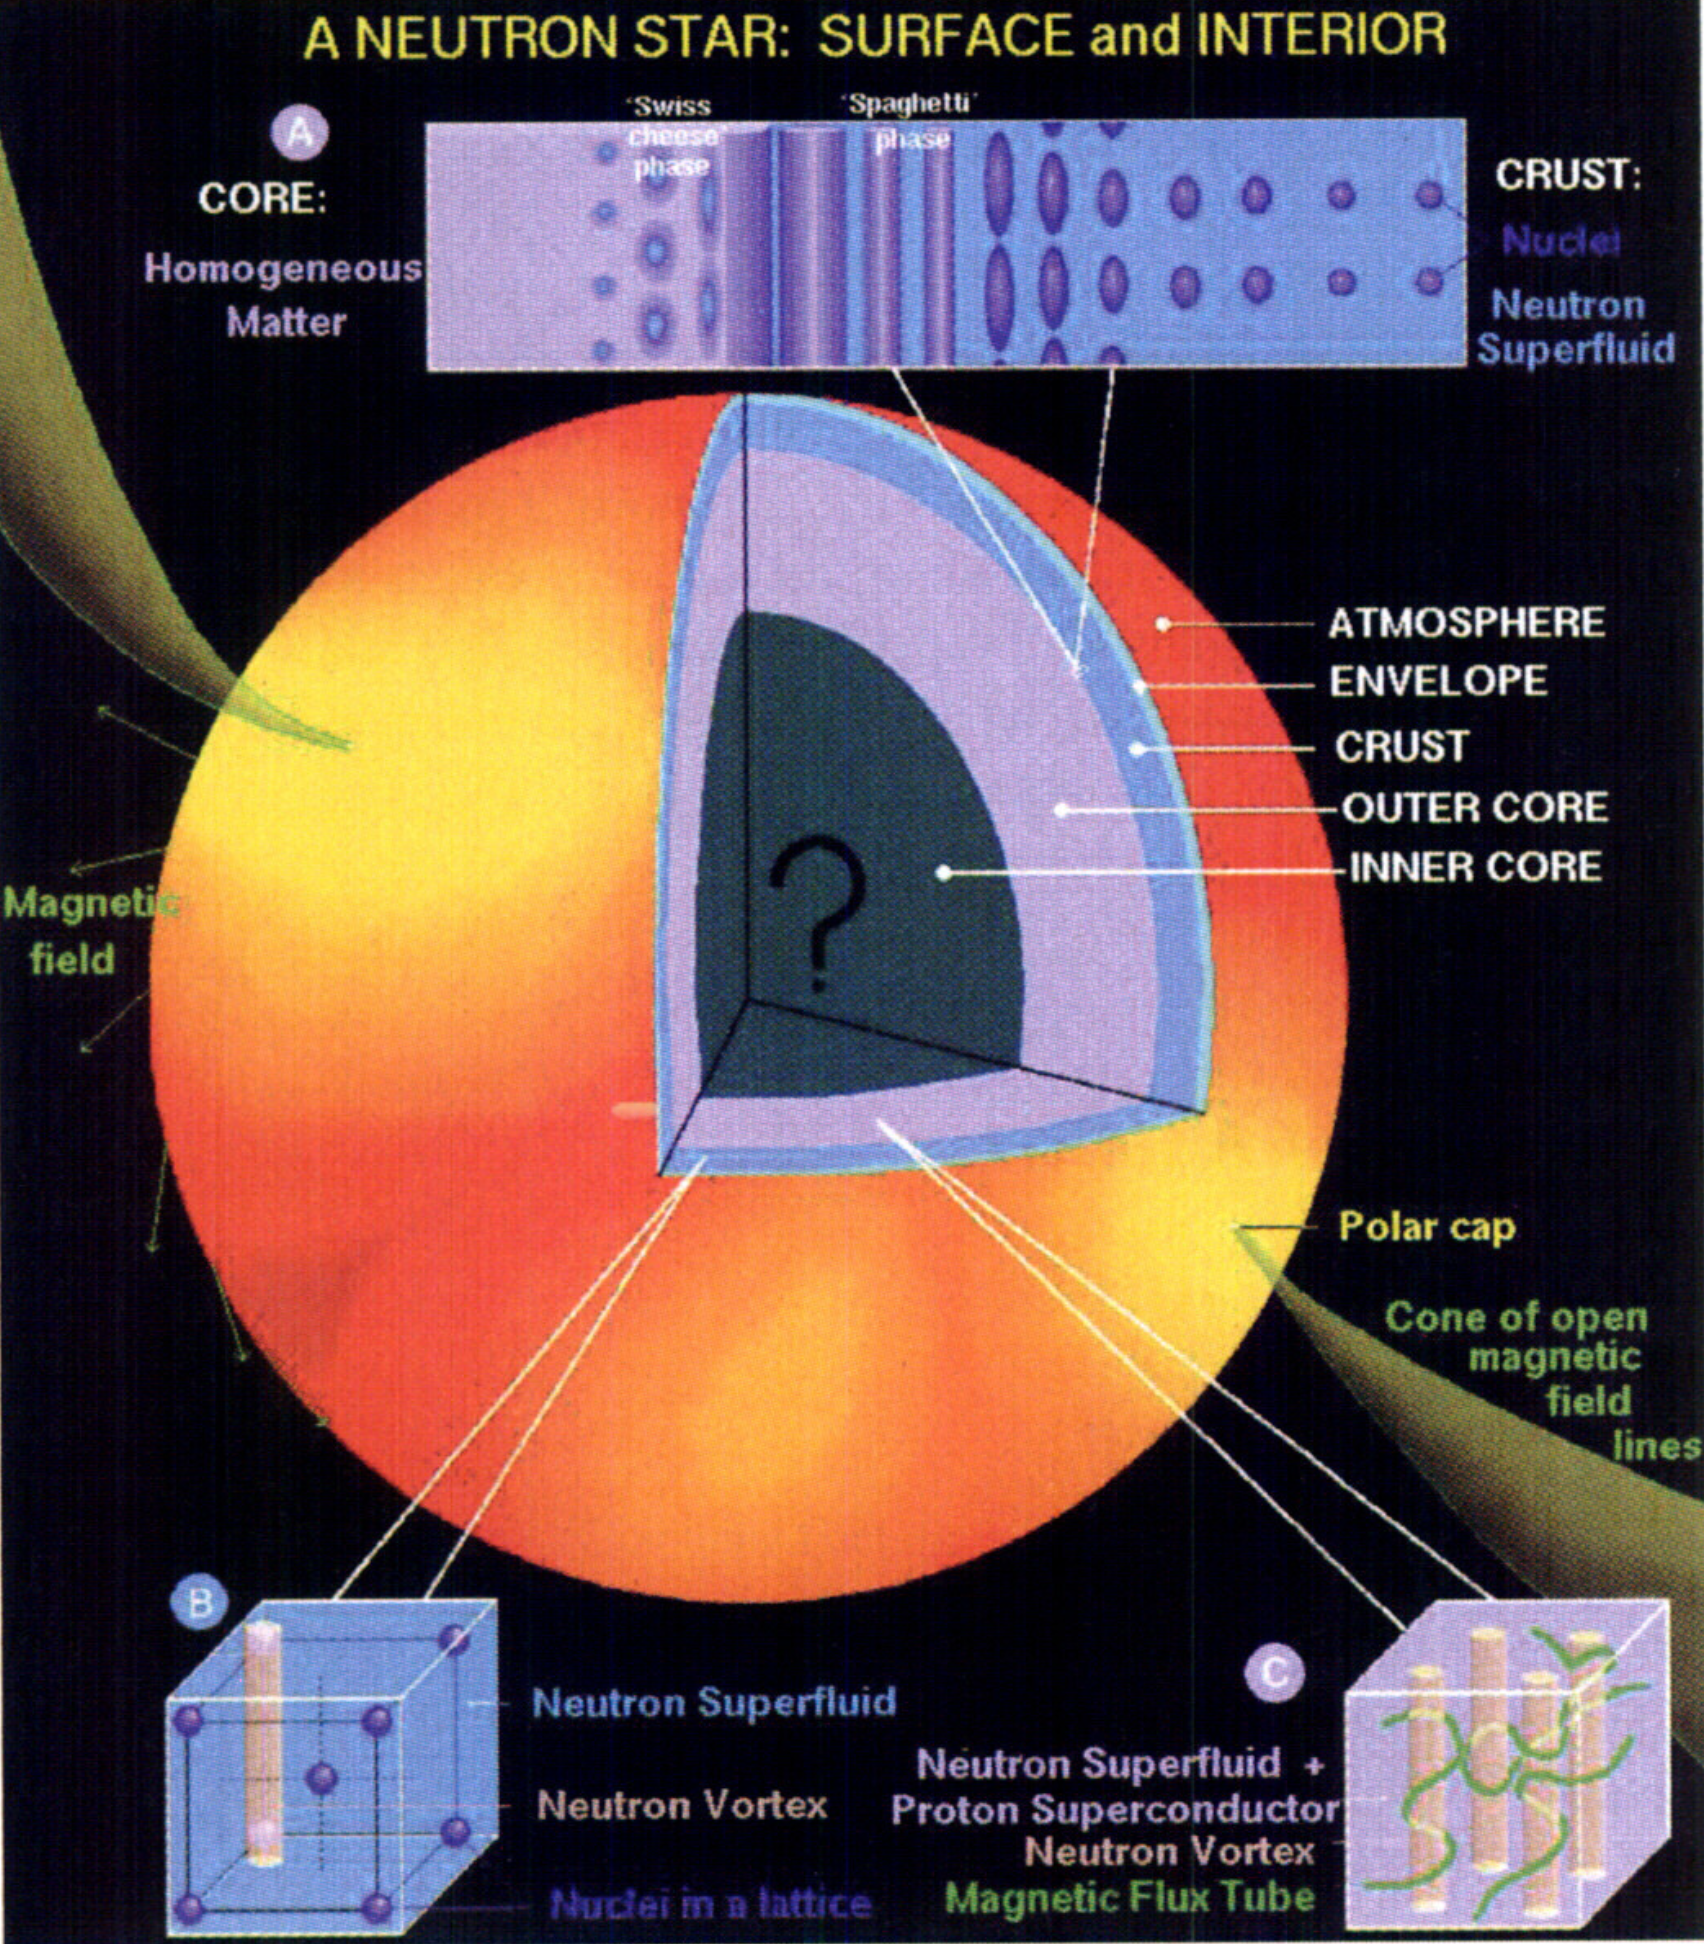
\includegraphics[width=.5\textwidth]{neutron star diagram.png}
    \caption{The major regions and possible composition inside a normal-matter neutron star. Top bar: illustrates the expected geometric compositions from homogenous matter at high densities in the core to nuclei at low densities.
    Superfluid aspects of the crust and outer core are shown in the insets [Figure courtesy of D. Page] \protect\cite{neutronstars}.}
    \label{fig:1}
\end{figure}

Neutron stars are created from the death of stars \cite{neutronstars2}: gravitational collapses in the core of a massive star ($>8 \: M_{\odot}$), triggering a Type II supernova explosion, and the core collapses cease when the interior density of the star reaches n$_0$ \cite{neutronstars}.
The proto-neutron star formed right after the supernova explosion rapidly shrinks as it emits neutrinos, thereby losing pressure. This loss of neutrinos forces the electrons and protons in the stellar interior to combine, making it a neutron-rich matter star \cite{neutronstars,neutronstars2,neutronstars3}. This proto-neutron stars only survive if they can stabilise the matter,
otherwise collapsing into a black hole \cite{neutronstars}.

A neutron star has 5 important regions: the inner and outer cores, the crust, the envelope, and the atmosphere (see Figure \ref{fig:1}) \cite{neutronstars}.
The atmosphere determines the characteristics of the emergent photon spectrum, while the envelope is essential in regulating the thermal energy transport and release from the star's surface, though both have negligible mass \cite{neutronstars}.
The crust primarily contains neutron-rich nuclei that varies depending on the density within the crust. At lower densities a lattice of voids can be formed as the nuclear lattice turns inside-out, which is eventually squeezed out in nuclear pasta transitions \cite{neutronstars}.
The superfluid in the crust could form a resevoir of angular momentum that could result in the pulsar glitch phenomena \cite{neutronstars}.

\subsection{Pulsars}

Pulsars are clocklike sources of highly periodic radiation emissions and extremely strong magnetic fields from spinning neutron stars. They provided valuable tools for investigating topics like neutron star interiors, globular cluster dynamics, the structure of the interstellar medium, and gravitational physics \cite{pulsars}.
The compositional aspects of neutron stars are what account for the high spinning velocities and stability of the periods found with pulsars \cite{pulsars}. The combination of the strong magnetic field and high rotational speed results in pulsars being efficient dynamos, generating incredibly strong electric fields of up to $10^{12}$ V cm$^{-1}$ or more at the surface \cite{pulsars}.
This causes an avalanche of electron-positron pairs to be ejected at high speeds as radiation beams at the neutron's stars poles (see Figure \ref{fig:3}) \cite{pulsars,pulsars2,pulsars3}. Eventually these pulsars lose energy through either magnetic dipole radiation or to charged particle winds, which leads to an increase in the spin period \cite{pulsars}.

\begin{figure}[!b]
    \centering
    \includegraphics[width=.8\textwidth]{artist rendition pulsar.jpeg}
    \caption{Artist's rendition of a pulsar. White thin lines describe axis of magnetic dipole. Cyan collimated twin lines represent pulsar emission. Red rotating disc describes magnetospheric activity. 3D model \protect\cite{artistpulsar}.}
    \label{fig:3}
\end{figure}

Pulsars generally have periods of about $\sim$1 s, but there also exist pulsars with periods less than $\sim$20 ms that are known as millisecond pulsars (MSPs) \cite{pulsars}.
It is theorised that MSPs undergo a recycling process, transferring mass and angular momentum from an aging and slowly rotating binary companion pulsar \cite{pulsars,pulsars3}. There exist about 1500 known pulsars, 90 of which are MSPs and half of those known MSPs are found in globular clusters:
compact and highly concentrated spheres of stars \cite{pulsars}. Most pulsars are only detectable at radio wavelength ranges, but younger pulsars tend to be detectable at optical, x-ray, and gamma-ray wavelengths \cite{pulsars}.

Many of these younger pulsars are surrounded by pulsar wind nebulae (PWNs), spin-down axis luminosities that are directly observable which allows for observations of the electrodynamics of pulsar magnetospheres \cite{pulsars}.
Theoretical models have previously described the PWNs as expanding spherical bubbles of relativistic gas confined by the surrounding medium, but recent x-ray, optical, and radio images of young pulsars have revealed a more intricate structure \cite{pulsars}.
Chandra x-ray images of the Crab and Vela pulsars (see Figure \ref{fig:2}) display toroidal and jet-like features, indicating that the pulsar winds are far from being isotropic \cite{pulsars}. For both these pulsars, the observed x-ray data suggests that the projected rotational axis closely matches the pulsar's projected direction of space velocity \cite{pulsars}.

\begin{figure}[H]
    \centering
    \begin{subfigure}[b]{.49\textwidth}
        \centering
        \includegraphics[width=\linewidth]{crab pwn.png}
        \caption{Crab Pulsar PWN}
        \label{fig:2a}
    \end{subfigure}
    \hfill
    \begin{subfigure}[b]{.485\textwidth}
        \centering
        \includegraphics[width=\linewidth]{vera pwn.png}
        \caption{Vela Pulsar PWN}
        \label{fig:2b}
    \end{subfigure}
    \caption{Chandra x-ray images of the PWNs surrounding the (\subref{fig:2a}) Crab and (\subref{fig:2b}) Vela pulsars \protect\cite{pulsars}}
    \label{fig:2}
\end{figure}

\subsection{Interstellar Dispersion} \label{sec:1.4}

Interstellar dispersion is the interaction of pulsar radio waves with free electrons in the interstellar medium (ISM), manifesting observationally as "stretched" pulses \cite{interstellardispersion,keith2013measurement,interstellardispersion2}. In the presence of protons and electrons, the low frequency radio waves of a pulsar are delayed in its propagation of light more than a higher frequency would \cite{interstellardispersion}.
The degree of this effect is known as the dispersion measure (DM), representing the free electron density between the source of the pulsar and the observer \cite{interstellardispersion,keith2013measurement}.

The DM of a pulsar can vary with time due to different factors, such as solar wind, relative motion to the observer, the terrestrial ionosphere, and the dynamics of the electrons and protons present in the ISM \cite{keith2013measurement,interstellardispersion2}. The DM can cause discrepancies in utilising MSPs as celestial clocks, so propagations in the pulses must be accounted for \cite{keith2013measurement}.

To calculate the DM, it must first be understood that, in general, electromagnetic radiation velocity is proportional to the square of the frequency divided by the electron density \cite{UCDpulsars},

\vspace{-2ex}
\begin{gather} \label{eq:1}
    v = \frac{f^2}{4150 \cdot n_e}
\end{gather}

where $v$ is the velocity, $f$ is the frequency, and $n_e$ is the electron density. In this report, a uniform interstellar electron density of 0.03 electrons cm$^{-3}$ is assumed. Therefore, Eq. \ref{eq:1} becomes:

\vspace{-2ex}
\begin{gather}
    v = \frac{f^2}{124.5}
\end{gather}

Noting t$_1$ (s) as the time of arrival of the pulsar with radio frequency f$_1$ (MHz), and t$_2$ (s) as the time of arrival of the \textit{same} pulsar with radio frequency f$_2$ (MHz), then the distance D (pc) can be derived as follows \cite{UCDpulsars,interstellardispersion},

\vspace{-2ex}
\begin{gather} \label{eq:3}
    t_2 - t_1 = 124.5 \cdot D \left[ \left( \frac{1}{f_2} \right)^2 - \left( \frac{1}{f_1} \right)^2 \right] \qquad \implies \qquad D = \frac{t_2 - t_1}{124.5 \left[ \left( \frac{1}{f_2} \right)^2 - \left( \frac{1}{f_1} \right)^2 \right]}
\end{gather}

Additionally, the DM is related to D by the interstellar electron density, $DM = n_e \: D$ \cite{interstellardispersion}.

\subsection{Radio Astronomy}

Radio astronomy studies and observes radio waves emitted by celestial objects \cite{radioastro,TAN20203}. By studying the radio wavelength range alongside the optical range, astronomers are able to get a borader understanding of celestial objects \cite{radioastro,TAN20203}.
Unlike optical light, radio waves are able to pass through dense dust and gas clouds, which allows radio telescopes to observe ragions of the universe otherwise obscured in the optical spectrum \cite{TAN20203}.
This allows for radio astronomy to be done both day and night, unobstructed even by Earth's atmosphere \cite{TAN20203}. Radio telescopes, similar in shape to a satellite TV dish but much larger, are able to produce images through the data converted and processed from the travelling radio waves \cite{radioastro}.
These images, as they are not taken in the visible spectrum, can be coloured in ways that represent different aspects, like temperature, "clumpiness", or the strength of the radio emissions \cite{radioastro}.
For example, the PWN images of the Crab and Vela pulsars (see Figure \ref{fig:2}) are coloured based on energy emission intensity.

\newpage

\section{Methodology} \label{sec:2}

This experiment made use of the \textit{Contemporary Laboratory Experiences in Astronomy (CLEA)} software provides a simulated observatory telescope. The "Radio Astronomy of Pulsars" program includes "Radio Telescope" and a "Data Analysis" mode for gathering and analysing pulsar data respectively.

The radio telescope was simulated to be located at the Gettysburg College Radio Observatory, Arizona, USA, and was pointed at a list of pre-selected pulsars for characterisation and analysis, though the option to locate the 500 pulsars available was also allowed. A radio receiever was included on the telescope,
allowing for pulsar data collection between the ranges of 400 to 1400 MHz. Variations to amplification (Vert. Gain) and sweep (Horz. Secs.) were also made available to maximise findings for further analysis.

\subsection{Investigation I: Observation of a Pulsar with a Single-Channel Radio Receiver}

The 0628-28 Pulsar was selected for analysis from the Hot List for this section of the experiment. Utilising the radio receiver, a trace graph plot of signal strength against time is shown. 
The most optimal setting for the gathering of data for this pulsar at 600 MHz was shown to be the vertical gain at 4 and the horizontal seconds at 4. The period of this pulsar could then be calculated by comparing the tie difference between two adjacent signal spikes or,
alternatively, increasing the horizontal seconds to 16 and measuring 10 pulses, calculcating the time difference between them, and then dividing by 10.

\subsection{Investigation II: The Periods of Different Pulsars}

The periods of different pulsars included in the Hot List were investigated for this section using the radio receiver, particularly the 2154+40, 0740-28, and 0531+21 pulsars alongside the previously studied 0628-28 pulsar. As this selection of pulsars had different periods and signal strengths, different behaviours and characteristics of pulsars were able to be investigated.
The periods of these pulsars were calculated similarly to Investigation I through the method of choice, making sure the vertical gain and horizontal seconds were optimised for each pulsar.

\subsection{Investigation III: Measurement of the Distance of Pulsars Using Disperion}

For this investigation the method of dispersion was used to find the distance to the pulsars, as covered in §\ref{sec:1.4}. Multiple readings of the 0628-28 pulsar were taken in 10 MHz increments over time from 400 to 600 MHz and 800 MHz, taken simulatenously over the same horizontal seconds for analytic comparison. By taking the readings up in 10 MHz the different traces could be aligned.

\newpage

\section{Results and Discussion} \label{sec:3}

\subsection{Investigation I: Observation of a Pulsar with a Single-Channel Radio Receiver}

The celestial coordinates of the 0628-28 pulsar are RA(6h 30m 49.5s), DEC(-28$^{\circ}$ 34' 44"), located on the Southern Hemisphere. Through the first method of period measurement with adjacent pulses for 600 MHz, the following was found,

\vspace{-2ex}
\[
\left.
\begin{aligned}
T_1 &= 0.56\,\text{s} \\
T_2 &= 1.81\,\text{s}
\end{aligned}
\quad \right\}
\quad T_2 - T_1 = 1.25\,\text{s}
\]

So the period of the 0628-28 pulsar is found to be \textbf{1.25 s} by measuring the time difference between two adjacent pulses. Comapring to the second method done over 10 pulses for 600 MHz, which is found to be,

\vspace{-2ex}
\[
\left.
\begin{aligned}
T_0 &= 0.12\,\text{s} \\
T_{10} &= 12.56\,\text{s}
\end{aligned}
\quad \right\}
\quad \frac{T_{10} - T_0}{10} = 1.244\,\text{s}
\]

Therefore the period of the 0628-28 pulsar is found to be \textbf{1.244 s} by measuring over 10 pulses and finding the time difference. The answer with both methods is found to be very similar, with the second method beign accurate to a slightly greater degree.

The same methods were used to find the period of a pulse over different freuqencies, which returned similar periods. Results were tabulated (Table \ref{tab:1}), done through the first method of measurement and calculating the uncertainties with subtraction error propagation, $\Delta P = \sqrt{(\Delta T_2)^2 + (\Delta T_1)^2}$.

\begin{table}[H]
    \centering
    \caption{Table of 0628-28 pulsar periods with uncertainties.}
    \label{tab:1}
    \resizebox{\textwidth}{!}{%
        \begin{tabular}{|
        >{\columncolor[HTML]{EFEFEF}}c |c|c|c|c|}
        \hline
        \textbf{Frequency (f) (MHz)} & \textbf{$T_1$ (s) $\pm$ 0.02 s} & \textbf{$T_2$ (s) $\pm$ 0.02 s} & \textbf{\# of Periods} & \textbf{Period of Pulsar (s) $\pm$ 0.0283 s} \\ \hline
        \textbf{400}  & 0.36 & 1.59 & 2 & 1.23 \\ \hline
        \textbf{600}  & 0.30 & 1.54 & 2 & 1.24 \\ \hline
        \textbf{800}  & 1.20 & 2.46 & 2 & 1.26 \\ \hline
        \textbf{1000} & 0.76 & 2.00 & 2 & 1.24 \\ \hline
        \textbf{1200} & 2.30 & 3.54 & 2 & 1.24 \\ \hline
        \textbf{1400} & 1.04 & 2.28 & 2 & 1.24 \\ \hline
        \end{tabular}%
    }
\end{table}

Reading the trace graph of the radio receiver it was observed that the signal was stronger at lower frequencies, so the ideal frequency range for detecting pulsars would be between 400 and 600 MHz. This allows for visible pulses with defined peaks, making it easier to calculate the time difference between pulses and find the pulsar period.

\subsection{Investigation II: The Periods of Different Pulsars}

The same method of period calculations through time difference between pulses of a pulsar as was done for Investigation I was used to measure the pulsar period for the 2154+40, 0740-28, and 0531+21 pulsars. Results were tabulated in Table \ref{tab:2}.

\begin{table}[H]
    \centering
    \caption{Table of different pulsar periods with uncertainties and relative strengths.}
    \label{tab:2}
    \resizebox{\textwidth}{!}{%
        \begin{tabular}{|
        >{\columncolor[HTML]{EFEFEF}}c |c|c|c|c|c|
        >{\columncolor[HTML]{EFEFEF}}c |}
        \hline
        \textbf{Pulsar} &
        \textbf{Frequency (f)} &
        \textbf{\begin{tabular}[c]{@{}c@{}}$T_1$ (s) \\ $\pm$ 0.02 s\end{tabular}} &
        \textbf{\begin{tabular}[c]{@{}c@{}}$T_2$ (s) \\ $\pm$ 0.02 s\end{tabular}} &
        \textbf{\# of Periods} &
        \textbf{\begin{tabular}[c]{@{}c@{}}Period of Pulsar (s) \\ $\pm$ 0.0283 s\end{tabular}} &
        \textbf{\begin{tabular}[c]{@{}c@{}}Relative\\ Strength\end{tabular}} \\ \hline
        \textbf{2154+40} & 400 MHz & 0.76   & 2.28   & 2 & 1.52  & Strong       \\ \hline
        \textbf{0740-28} & 600 MHz & 0.1875 & 0.3550 & 2 & 0.17  & V. Strong    \\ \hline
        \textbf{0531+21} & 800 MHz & 0.2975 & 0.3325 & 2 & 0.035 & V. V. Strong \\ \hline\hline
        \textbf{0628-28} & 600 MHz & 0.30   & 1.54   & 2 & 1.24  & -            \\ \hline
        \end{tabular}%
    }
\end{table}

Reading the pulsar periods from Table \ref{tab:2}, it is clear to see which pulsars are younger and older. Arranging them for visibility,

\vspace{-2ex}
\[
\begin{aligned}
\text{\textbf{YOUNGEST}} \qquad & 0531+21 \\
& 0740-28 \\
& 0628-28 \\
\text{\textbf{OLDEST}} \qquad & 2154+40
\end{aligned}
\]

This aligns well with what would be expected as the 0531+21 pulsar is the Crab Nebula Pulsar, which is young and powerful.

\vspace{1cm}
\subsection{Investigation III: Measurement of the Distance of Pulsars Using Disperion}

The distance in parsecs from the observer to the pulsar was calculared using Eq. \ref{eq:3}. This process was done for both the 0628-28 and the 2154-40 pulsars and tabulated (Table \ref{tab:4} and Table \ref{tab:5}, respectively).

For the 0628-28 pulsar, the following times were found for a pulse at 3 different frequencies: 400 MHz, 600 MHz, and 800 MHz. These were:

\vspace{-2ex}
\begin{gather*}
    \mathbf{T_{400}} \; : \quad 3.11 \pm 0.02 \:\text{s} \qquad\qquad \mathbf{T_{600}} \; : \quad 2.61 \pm 0.02 \:\text{s} \qquad\qquad \mathbf{T_{800}} \; : \quad 2.435 \pm 0.02 \:\text{s}
\end{gather*}

\begin{table}[H]
    \centering
    \caption{Distance to the 0628-28 pulsar through dispersion analysis using Eq. \ref{eq:3}.}
    \label{tab:3}
    \resizebox{.7\textwidth}{!}{%
        \begin{tabular}{|
        >{\columncolor[HTML]{EFEFEF}}c 
        >{\columncolor[HTML]{EFEFEF}}c |ccc}
        \cline{1-2}
        \multicolumn{2}{|c|}{\cellcolor[HTML]{EFEFEF}\textbf{Frequencies}} &
        &
        &
        \\ \hline
        \multicolumn{1}{|c|}{\cellcolor[HTML]{EFEFEF}\textbf{f$_1$}} &
        \textbf{f$_2$} &
        \multicolumn{1}{c|}{\textbf{T$_2$-T$_1$ (s) $\pm$ 0.0283 s}} &
        \multicolumn{1}{c|}{\textbf{(1/f$_2$)$^2$ - (1/f$_1$)$^2$}} &
        \multicolumn{1}{c|}{\textbf{D (pc)}} \\ \hline
        \multicolumn{1}{|c|}{\cellcolor[HTML]{EFEFEF}600} &
        400 &
        \multicolumn{1}{c|}{0.5} &
        \multicolumn{1}{c|}{3.47 $\times$ 10$^{-6}$} &
        \multicolumn{1}{c|}{1157.37} \\ \hline
        \multicolumn{1}{|c|}{\cellcolor[HTML]{EFEFEF}800} &
        400 &
        \multicolumn{1}{c|}{0.675} &
        \multicolumn{1}{c|}{4.6875 $\times$ 10$^{-6}$} &
        \multicolumn{1}{c|}{1156.63} \\ \hline
        \multicolumn{1}{|c|}{\cellcolor[HTML]{EFEFEF}800} &
        600 &
        \multicolumn{1}{c|}{0.175} &
        \multicolumn{1}{c|}{1.2153 $\times$ 10$^{-6}$} &
        \multicolumn{1}{c|}{1156.61} \\ \hline
        \end{tabular}%
    }
\end{table}

As the distances calculated for the 0628-28 pulsar agree to at least two significant figures, it can be said that the calculations agree with each other. Taking the average of the three distances, it can be assumed that this pulsar is approximately \textbf{1156.87 pc} away from Earth.

For the 2154+40 pulsar, the following times were found for a pulse at 3 different frequencies: 400 MHz, 600 MHz, and 800 MHz. These were:

\vspace{-2ex}
\begin{gather*}
    \mathbf{T_{400}} \; : \quad 5.32 \pm 0.02 \:\text{s} \qquad\qquad \mathbf{T_{600}} \; : \quad 4.30 \pm 0.02 \:\text{s} \qquad\qquad \mathbf{T_{800}} \; : \quad 3.94 \pm 0.02 \:\text{s}
\end{gather*}

\begin{table}[H]
    \centering
    \caption{Distance to the 2154+40 pulsar through dispersion analysis using Eq. \ref{eq:3}.}
    \label{tab:4}
    \resizebox{.7\textwidth}{!}{%
        \begin{tabular}{|
        >{\columncolor[HTML]{EFEFEF}}c 
        >{\columncolor[HTML]{EFEFEF}}c |ccc}
        \cline{1-2}
        \multicolumn{2}{|c|}{\cellcolor[HTML]{EFEFEF}\textbf{Frequencies}} &
        &
        &
        \\ \hline
        \multicolumn{1}{|c|}{\cellcolor[HTML]{EFEFEF}\textbf{f$_1$}} &
        \textbf{f$_2$} &
        \multicolumn{1}{c|}{\textbf{T$_2$-T$_1$ (s) $\pm$ 0.0283 s}} &
        \multicolumn{1}{c|}{\textbf{(1/f$_2$)$^2$ - (1/f$_1$)$^2$}} &
        \multicolumn{1}{c|}{\textbf{D (pc)}} \\ \hline
        \multicolumn{1}{|c|}{\cellcolor[HTML]{EFEFEF}600} &
        400 &
        \multicolumn{1}{c|}{1.02} &
        \multicolumn{1}{c|}{3.47 $\times$ 10$^{-6}$} &
        \multicolumn{1}{c|}{2361.03} \\ \hline
        \multicolumn{1}{|c|}{\cellcolor[HTML]{EFEFEF}800} &
        400 &
        \multicolumn{1}{c|}{1.38} &
        \multicolumn{1}{c|}{4.6875 $\times$ 10$^{-6}$} &
        \multicolumn{1}{c|}{2364.66} \\ \hline
        \multicolumn{1}{|c|}{\cellcolor[HTML]{EFEFEF}800} &
        600 &
        \multicolumn{1}{c|}{0.36} &
        \multicolumn{1}{c|}{1.2153 $\times$ 10$^{-6}$} &
        \multicolumn{1}{c|}{2379.30} \\ \hline
        \end{tabular}%
    }
\end{table}

The distances calculated for the 2154+40 pulsar do not fully agree to two significant figures. The reason for the disagreements might be from error in measuring pulse peaks on the trace graphs, and the results could have been made more accurate if they were taken over a broader frequency range.
Physical factors that could have affected the distance calculation accuracies is non-uniform interstellar dispersion. However, still taking the average of these distances, the 2154-40 pulsar is approximately \textbf{2368.33 pc} from Earth.

\subsubsection{Optional Investigation: The Distance to Short-Period Pulsars}

The same method for measuring the distance to short-period pulsars 0740-28 and 0531+21 through interstellar disperion was used for calculations and tabulated in Table \ref{tab:5} and Table \ref{tab:6} respectively.

For the 0740-28 pulsar, the following times were found for a pulse at 3 different frequencies: 800 MHz, 1000 MHz, and 1200 MHz. These were:

\vspace{-2ex}
\begin{gather*}
    \mathbf{T_{800}} \; : \quad 0.315 \pm 0.02 \:\text{s} \qquad\qquad \mathbf{T_{1000}} \; : \quad 0.145 \pm 0.02 \:\text{s} \qquad\qquad \mathbf{T_{1200}} \; : \quad 0.050 \pm 0.02 \:\text{s}
\end{gather*}

\begin{table}[H]
    \centering
    \caption{Distance to the 0740-28 pulsar through dispersion analysis using Eq. \ref{eq:3}.}
    \label{tab:5}
    \resizebox{.7\textwidth}{!}{%
        \begin{tabular}{|
        >{\columncolor[HTML]{EFEFEF}}c 
        >{\columncolor[HTML]{EFEFEF}}c |ccc}
        \cline{1-2}
        \multicolumn{2}{|c|}{\cellcolor[HTML]{EFEFEF}\textbf{Frequencies}} &
        &
        &
        \\ \hline
        \multicolumn{1}{|c|}{\cellcolor[HTML]{EFEFEF}\textbf{f$_1$}} &
        \textbf{f$_2$} &
        \multicolumn{1}{c|}{\textbf{T$_2$-T$_1$ (s) $\pm$ 0.0283 s}} &
        \multicolumn{1}{c|}{\textbf{(1/f$_2$)$^2$ - (1/f$_1$)$^2$}} &
        \multicolumn{1}{c|}{\textbf{D (pc)}} \\ \hline
        \multicolumn{1}{|c|}{\cellcolor[HTML]{EFEFEF}1000} &
        800 &
        \multicolumn{1}{c|}{0.17} &
        \multicolumn{1}{c|}{5.625 $\times$ 10$^{-7}$} &
        \multicolumn{1}{c|}{2427.49} \\ \hline
        \multicolumn{1}{|c|}{\cellcolor[HTML]{EFEFEF}1200} &
        800 &
        \multicolumn{1}{c|}{0.265} &
        \multicolumn{1}{c|}{8.681 $\times$ 10$^{-7}$} &
        \multicolumn{1}{c|}{2451.92} \\ \hline
        \multicolumn{1}{|c|}{\cellcolor[HTML]{EFEFEF}1200} &
        1000 &
        \multicolumn{1}{c|}{0.095} &
        \multicolumn{1}{c|}{3.056 $\times$ 10$^{-7}$} &
        \multicolumn{1}{c|}{2496.90} \\ \hline
        \end{tabular}%
    }
\end{table}

For the 0531+21 Crab Nebula pulsar, the following times were found for a pulse at 3 different frequencies: 800 MHz, 1000 MHz, and 1200 MHz. These were:

\vspace{-2ex}
\begin{gather*}
    \mathbf{T_{400}} \; : \quad 0.095 \pm 0.02 \:\text{s} \qquad\qquad \mathbf{T_{600}} \; : \quad 0.065 \pm 0.02 \:\text{s} \qquad\qquad \mathbf{T_{800}} \; : \quad 0.025 \pm 0.02 \:\text{s}
\end{gather*}

\begin{table}[H]
    \centering
    \caption{Distance to the 0531+21 (Crab Nebula) pulsar through dispersion analysis using Eq. \ref{eq:3}.}
    \label{tab:6}
    \resizebox{.7\textwidth}{!}{%
        \begin{tabular}{|
        >{\columncolor[HTML]{EFEFEF}}c 
        >{\columncolor[HTML]{EFEFEF}}c |ccc}
        \cline{1-2}
        \multicolumn{2}{|c|}{\cellcolor[HTML]{EFEFEF}\textbf{Frequencies}} &
        &
        &
        \\ \hline
        \multicolumn{1}{|c|}{\cellcolor[HTML]{EFEFEF}\textbf{f$_1$}} &
        \textbf{f$_2$} &
        \multicolumn{1}{c|}{\textbf{T$_2$-T$_1$ (s) $\pm$ 0.0283 s}} &
        \multicolumn{1}{c|}{\textbf{(1/f$_2$)$^2$ - (1/f$_1$)$^2$}} &
        \multicolumn{1}{c|}{\textbf{D (pc)}} \\ \hline
        \multicolumn{1}{|c|}{\cellcolor[HTML]{EFEFEF}1000} &
        800 &
        \multicolumn{1}{c|}{0.03} &
        \multicolumn{1}{c|}{5.625 $\times$ 10$^{-7}$} &
        \multicolumn{1}{c|}{428.38} \\ \hline
        \multicolumn{1}{|c|}{\cellcolor[HTML]{EFEFEF}1200} &
        800 &
        \multicolumn{1}{c|}{0.07} &
        \multicolumn{1}{c|}{8.681 $\times$ 10$^{-7}$} &
        \multicolumn{1}{c|}{647.68} \\ \hline
        \multicolumn{1}{|c|}{\cellcolor[HTML]{EFEFEF}1200} &
        1000 &
        \multicolumn{1}{c|}{0.04} &
        \multicolumn{1}{c|}{3.056 $\times$ 10$^{-7}$} &
        \multicolumn{1}{c|}{1051.33} \\ \hline
        \end{tabular}%
    }
\end{table}

The distances calculated for the 0740-28 and Crab Nebula Pulsar are also not seen to agree to two significant figures, though as they are both relatively young pulsars, there is a physical explanation as to why they might not agree.
Since the pulsars are quite young, they are more susceptible to glitches (as discussed in §\ref{sec:1.2}) where the rotational speed of the pulsar may suddenly increase, affecting timings. Beacause of the youthfulness there may also be discrepancies in pulse peak shaprness and greater timing noise due
to the pulsar's high rotational speed and energy, making it unstable. Observational errors could be due to the frequency range being too high, causing the denominator of the distance-disperion Eq. \ref{eq:3} to become too big relative to the numerator, causing a higher difference between the distances calculated.
An assumption for the distance to the pulsars can be taken from the averages of the values, resulting in \textbf{2458.77 pc} of the 0740-28 pulsar from the Earth, and \textbf{709.13 pc} of the 0531+21 pulsar from the Earth.

Additionally, to the Crab Nebula pulsar, since its rotational speed is so incredibly high that my time differences were 0.03, 0.07, and 0.04, it means that in a trace graph it is incredibly difficult to accurately choose the peaks of the pulses. This caused huge errors in the calculations of the distances.
To accommodate for the Crab Nebula's short period and fast rotation, results could have been taken in higher frequencies beyond what was offered with the radio telescope. X-ray telescopes, like the one that took the PWN pictures seen in Figure \ref{fig:3}, are much better for accurately capturing short-period pulsars like the ones investigated.
However, it is not possible to use the dispersion-distance equation with X-rays, so the distances would have had to be found in other ways. Regardless, overlapping issues with short-period pulsars are prevalent in the measurements above.

\newpage

\section{Conclusion} \label{sec:4}

The experiments done in this report confirmed multiple aspects for pulsars that were being investigated, such as the period of pulsars and the distance to them in parsecs.

The investigations on the periods of 4 different pulsars (0628-28, 2154+40, 0740-28, and 0531+21 (Crab Nebula)) returned very different values in seconds that were then arranged from youngest to oldest.
The youngest pulsar was the Crab Nebula 0531+21 pulsar with a period of \textbf{0.035 s}, followed by the 0740-28 pulsar with a period of \textbf{0.17 s}, then the 0628-28 pulsar with a period of \textbf{1.24 s}, and lastly the 2154+40 pulsar with a period of \textbf{1.52 s}.
This aligned well with expectations as the Crab Nebula is the youngest pulsar between those. Future renditions of this experiment could be done to a higher degree of accuracy by counting the period over a greater amount of pulses with the second method of calculation.

The investigations of the distances to the pulsars with the disperion method for the same 4 pulsars as before, the 2 long-period pulsars (0628-28 and 2154+40) and the 2 short-period pulsars (0740-28 and 0531+21). The approximate distances were determined through the average of several
calculated distances. 

For the long-period pulsars, the average distances were \textbf{1156.87 pc} and \textbf{2368.33 pc} for the 0628-28 and 2154+40 pulsars respectively. These values are representative of the average over all the calculated distances with minor deviation, showing they agree with calculations. As long-period pulsars tend to be older,
they also tend to be more stable, providing good results for a low frequency range.

For the short-period pulsars, the average distances were \textbf{2458.77 pc} and \textbf{709.13 pc} for the 0740-28 and 0531+21 pulsars respectively. These values are not representative of the values calculated for different frequencies and there is great variation between the values resulting in a misleading average of the distance.
The likely causes of the variations of the values achieved for these distances could be due to the youth and therefore instability of the pulsars, resulting in noisy and overlapping pulses seen in a trace graph plot. Young short-period pulsars are also susceptible to glitches in which the rotational speed suddenly increases, leading to greater uncertainties
in the observations of the periods. 

\newpage

%%%%%%%%%%%%%%%%%%%%%%%%%%%%%%%%%%%

\bibliographystyle{IEEEtran}
\bibliography{References} \label{sec:ref}

\vspace{1.5cm}

\listoffigures

\listoftables

\end{document}